\section{Projected Sensitivity}
\par
As was shown in \autoref{sec:eft_theory}, the response from EFT operators extends significantly above the region of interest that the SI WIMP interaction lives in.
In this section the sensitivity to these responses is set for the planned full exposure of LZ, 1000 live-days with 5.6 tonne of xenon.
The approaches adopted in this section are analogously to \cite{LZ_projected_sensitivity_paper_ref}, but with with an extended region of interest.
The projected detector parameters are shown in \autoref{tab:projected_sensitivity_detector_parameters}.
\begin{table}[]
    \centering
    \begin{tabular}{c|c}
        Parameter   & Value  \\ \hline
        $g_{1}$     & 0.119 \\
        $g_{2}$     & 79.1  \\
        Drift field & 310 Vcm$^{-1}$ \\
        electron lifetime & 850 $\mu$s
    \end{tabular}
    \caption{Key detector parameters for the LXe-TPC parameters in the projected detector performance case.}
    \label{tab:projected_sensitivity_detector_parameters}
\end{table}
\par
The extended region of interest was set such that the it was below the end point of any calibration of NEST ($\backsim$ 300 keV from AmBe).
As such it was defined as S1$_c$ [3, 500].
This was determined from simulations of a flat NR background, which is shown in \autoref{fig:projected_detector_model_response_for_flat_nr}.
With the projected detector parameters, an S1$_c$ of 500 phd will be from pulses around 250 keV, but the largest recoil (within 3 $\sigma$) is from 278 keV recoils.

\begin{figure}[!htbp]%
\centering
    \begin{tikzpicture}
    \centering
        \begin{groupplot}[view={0}{90},
            group style = {group size = 2 by 1,
            horizontal sep=0.6cm}]
            \nextgroupplot[
            width=0.48\textwidth, height=8cm,
            xlabel={Recoil Energy [keV$_{NR}$]},
            ylabel={S1$_{c}$ [phd]},
            mark size=0pt,
            xmin=0, xmax=300,
            ymin=0, ymax=600]

            \addplot[yellow, name path = psig2] table[x=energy, y=psig2]
                      {Data/HENR/Projected_Sensitivity/data_cuts/s1_vs_recoil.dat};
            \addplot[yellow, name path = nsig2] table[x=energy, y=nsig2]
                      {Data/HENR/Projected_Sensitivity/data_cuts/s1_vs_recoil.dat};
            
            \addplot[green, name path = psig1] table[x=energy, y=psig1]
                      {Data/HENR/Projected_Sensitivity/data_cuts/s1_vs_recoil.dat};
            \addplot[green, name path = nsig1] table[x=energy, y=nsig1]
                      {Data/HENR/Projected_Sensitivity/data_cuts/s1_vs_recoil.dat};
                      
            \addplot[yellow, forget plot] fill between[of=nsig2 and psig2]; 
            \addplot[green, forget plot] fill between[of=nsig1 and psig1];
            
            \addplot[black] table[x=energy, y=mean]
                    {Data/HENR/Projected_Sensitivity/data_cuts/s1_vs_recoil.dat};
            
            \addplot[blue, dashed] coordinates { (0,500)  (325,500)};
            \addplot[black, dashed] coordinates { (278,0)  (278,700)};
                  
            \nextgroupplot[
            width=0.48\textwidth, height=8cm,
            xlabel={Recoil Energy [keV$_{NR}$]},
            ylabel={log$_{10}$(S2$_{c}$ [phd])},
            yticklabel pos=right,
            mark size=0pt,
            xmin=0, xmax=300,
            ymin=2.0, ymax=5.0]
            
            \addplot[yellow, name path = psig2] table[x=energy, y=psig2]
                      {Data/HENR/Projected_Sensitivity/data_cuts/logs2_vs_recoil.dat};
            \addplot[yellow, name path = nsig2] table[x=energy, y=nsig2]
                      {Data/HENR/Projected_Sensitivity/data_cuts/logs2_vs_recoil.dat};
            \addplot[yellow, forget plot] fill between[of=nsig2 and psig2];          
            
            \addplot[green, name path = psig1] table[x=energy, y=psig1]
                      {Data/HENR/Projected_Sensitivity/data_cuts/logs2_vs_recoil.dat};
            \addplot[green, name path = nsig1] table[x=energy, y=nsig1]
                      {Data/HENR/Projected_Sensitivity/data_cuts/logs2_vs_recoil.dat};
            \addplot[green, forget plot] fill between[of=nsig1 and psig1];
            
            \addplot[black] table[x=energy, y=mean]
                    {Data/HENR/Projected_Sensitivity/data_cuts/logs2_vs_recoil.dat};
                    
            \addplot[black, dashed] coordinates { (278,2)  (278,5)};
        
        \end{groupplot}
    \end{tikzpicture}
    \caption{Detector response in S1 (\textbf{Left}) and S2 (\textbf{Right}) space for a given recoil in the LZ detector assuming the projected detector parameters.
             The values have been extrapolated from simulations of a flat NR spectrum.
    }
    \label{fig:projected_detector_model_response_for_flat_nr}
\end{figure}

\subsection{Background Models}
\par
The background model considered was made up of 11 components which represent the most significant contributors discussed in \autoref{sec:lz_detector}.
Contributions from ``Detector components", ``Surface contamination" and ``Environmental" sources are summed together, but kept separate as ER and NR components.
This is performed as generally speaking the shape contribution is similar\footnote{this is particularly true in low energy recoil searches (<30 keV), where they all appear as flat contributions.}.
Neutrinos are se


\par
One background that was not considered are $\gamma$-X events.
These were excluded because in order to effectively model them the positional information of events need to be considered, and we have limited the observable parameters to \{S1$_c$,log$_{10}$(S2$_c$)\}. 
When LUX included 5-dimensions to in their PLR for a RUN-4 EFT analysis the resultant PLR required $\approx$15,000 CPU-hours per mass point \cite{billyboxer_thesis_ref} and so it was desirable to avoid a similar situation here.
There are novel ways of over coming this such detailed in \cite{flamenest_ref} and \cite{lux_ml_plr_ref}, but these would have required a significant effort to intergrate into the LZ computing framework.
In future searches, LZ is planning on using a boosted decision tree machine learning technique that is based upon LUX Run-4 EFT analysis \cite{LUX_RUN4_EFT_2021}.





\begin{enumerate}
    \item \textbf{SS}: Select events which have only scattered once, ``single scatter". An event is a single scatter in the TPC if the energy-weighted standard deviation of the deposits is less than the detector resolution. This is taken to be $\sigma_r <$ 3.0 cm and $\sigma_z <$ 0.2 cm.
    \item \textbf{ROI}: Select events where the recoil energy is in the range expected from a WIMP scatter and set on S1$_c$, S2 (uncorrected). This is cut is dependent upon which model of dark matter we are using. Here S1$_c$ must be less than 500 phd and have at least a 3-fold coincidence in the TPC PMTs. S2 must be greater than 415, the value required for at least 5 emitted electrons. This electron requirement is to ensure that the S2 size is large enough for position reconstruction.
    \item \textbf{FID}: The inner volume, or fiducial volume of the TPC is taken, removing events near the edges. The FID is defined as a cylinder extended from the centre of the TPC to 4 cm from the TPC walls, 2 cm above the cathode grid, and 13 cm below the gate grid. This inner volume contains 5.6 tonnes of LXe, meaning that there is 1.4 tonnes of xenon used for self-shielding.
    \item \textbf{Veto}: TPC scatters where there is a time-coincident deposit in either of the veto detectors are removed. In the Skin detector the signal must be within 800 $\mu$s of the TPC scatter and be at least 3 phd in size. In the OD the deposit must be at least 200 keV in size and within 500 $\mu$s of the TPC scatter. This OD selection was chosen to maintain consistency with \cite{LZ_projected_sensitivity_paper_ref} with an older simulation framework.
\end{enumerate}
The events that are left are then defined as as a differential rate per recoil energy can then be calculated for each component.
Other sources of backgrounds which would only scatter once anyway do not need to be simulated in this way, instead the rate can be determined directly from the flux and scattering cross-section.
The spectrial contributions from each of of the background components is shown in FIG XXX.
The expected number of events from each of these components in the WIMP-SI search region of interest and in the extended region used here are shown in 
\autoref{tab:projected_lz_backgrounds}.
A simulated dataset of these backgrounds is shown in  \autoref{fig:sensitivity_paper_backgrounds}.

\begin{table}[]
    \centering
    \begin{tabular}{c|c|c|c}
        \multirow{2}{*}{Background}                  & \multicolumn{2}{|c|}{N}                          & \multirow{2}{*}{$\sigma$/N}  \\ 
                                                     &  (S1$_c <$ 80 phd)     & (S1$_c <$ 500 phd)      &              \\ \hline
        \textbf{ER contributions}                    &                        &                         &   \\
        Detector contaminants                        & 171                    & 1166                    & 20\% \cite{LZ_projected_sensitivity_paper_ref}        \\
        pp + ${}^{7}$Be + ${}^{13}$N solar neutrinos & 615                    & 2950                    & 2\% \cite{pp_solar_neutrinos_rate_ref}       \\
        ${}^{222}$Rn                                 & 1915                   & 12514                   & 10\% \cite{lz_predicted_radon_rate_ref}        \\
        ${}^{220}$Rn                                 & 316                    & 1902                    & 10\% \cite{lz_predicted_radon_rate_ref}        \\
        ${}^{136}$Xe 2$\mu\beta\beta$                & 495                    & 19183                   & 50\% \cite{double_beta_decay_rate_ref}        \\
        ${}^{85}$Kr                                  & 83                     & 557                     & 20\% \cite{kr85_rate_ref}         \\ \hline
        \textbf{NR contributions}                    &                        &                         &   \\
        Detector contaminants                        & 0.81                   & 1.91                    & 20\% \cite{LZ_projected_sensitivity_paper_ref}         \\
        ${}^{8}$B solar neutrinos                    & 36                     & 36                      & 4\%  \cite{b8_neutrino_rate_ref}       \\
        hep solar neutrinos                          & 0.9                    & 0.9                     & 15\% \cite{solar_neutrinos_rate_ref, pp_solar_neutrinos_rate_ref}        \\
        Diffuse supernova neutrinos                  & 0.15                   & 0.15                    & 50\% \cite{dissuse_supernova_neutrinos_rate_ref}        \\
        Atmospheric neutrons                         & 0.65                   & 0.65                    & 25\% \cite{atmospheric_neutrinos_rate_ref}      
    \end{tabular}
    \caption{Backgrounds considered in the PLR for a projected sensitivity to EFT operator coupling. The values for the WIMP-SI search region values differ from previous studies \cite{LZ_projected_sensitivity_paper_ref,LZ_Ibles_LZStats_Thesis_ref}. This is due to an upgraded NEST package version used here.}
    \label{tab:projected_lz_backgrounds}
\end{table}

\begin{figure}[!htbp]%
\centering
    \begin{tikzpicture}
    \centering
        \begin{groupplot}[view={0}{90},
            group style = {group size = 2 by 1}]
            \nextgroupplot[
            width=0.5\textwidth, height=8cm,
            xlabel=Recoil Energy (keV),
            ylabel=Differential Rate (kg/day/keV),
            legend pos=north east,
            mark size=0pt,
            xmin=0, xmax=2700,
            ymode=log]
                \addplot
                    table[x=Energy,y=Rate]
                    {Data/HENR/Projected_Sensitivity/Background_Rates/detector_er.dat};
      %          \addlegendentry{Det. + Sur. + Env.};
      %         \addplot
      %             table[x=Energy,y=Rate]
      %             {Data/HENR/Projected_Sensitivity/Background_Rates/Xe136.dat};
      %          \addlegendentry{${}^{136}$Xe}
      %         \addplot
      %             table[x=Energy,y=Rate]
      %             {Data/HENR/Projected_Sensitivity/Background_Rates/Rn222.dat};
      %          \addlegendentry{${}^{222}$Rn};
      %         \addplot
      %             table[x=Energy,y=Rate]
      %             {Data/HENR/Projected_Sensitivity/Background_Rates/Rn220.dat};
      %          \addlegendentry{${}^{220}$Rn};
      %         \addplot
      %             table[x=Energy,y=Rate]
      %             {Data/HENR/Projected_Sensitivity/Background_Rates/Solar.dat};
      %          \addlegendentry{Solar $\nu$};
      %         \addplot
      %             table[x=Energy,y=Rate]
      %                {Data/HENR/Projected_Sensitivity/Background_Rates/Kr85.dat};
      %          \addlegendentry{${}^{85}$Kr};
                  
            \nextgroupplot[
            width=0.5\textwidth, height=8cm,
            xlabel=Recoil Energy (keV),
            yticklabel pos=right,
            legend pos=north east,
            mark size=0pt,
            xmin=0, xmax=250,
            ymin=1e-12, ymax=,
            ymode=log]
                \addplot
                    table[x=Energy,y=Rate]
                    {Data/HENR/Projected_Sensitivity/Background_Rates/detector_nr.dat};
                \addlegendentry{Det. + Sur. + Env.};
                \addplot
                    table[x=Energy,y=Rate]
                    {Data/HENR/Projected_Sensitivity/Background_Rates/atm.dat};
                \addlegendentry{Atm};
                \addplot
                    table[x=Energy,y=Rate]
                    {Data/HENR/Projected_Sensitivity/Background_Rates/DSN_DiffRate.dat};
                \addlegendentry{DSN};
                \addplot
                    table[x=Energy,y=Rate]
                    {Data/HENR/Projected_Sensitivity/Background_Rates/hep.dat};
           %     \addlegendentry{hep};
           %     \addplot
           %         table[x=Energy,y=Rate]
           %         {Data/HENR/Projected_Sensitivity/Background_Rates/B8.dat};
           %     \addlegendentry{${}^{8}$B}
        
        \end{groupplot}
    \end{tikzpicture}
    \caption{Backgrounds considered in the projected sensitivity.}
    \label{fig:sensitivity_paper_backgrounds}
\end{figure}

\begin{figure}
    \centering
    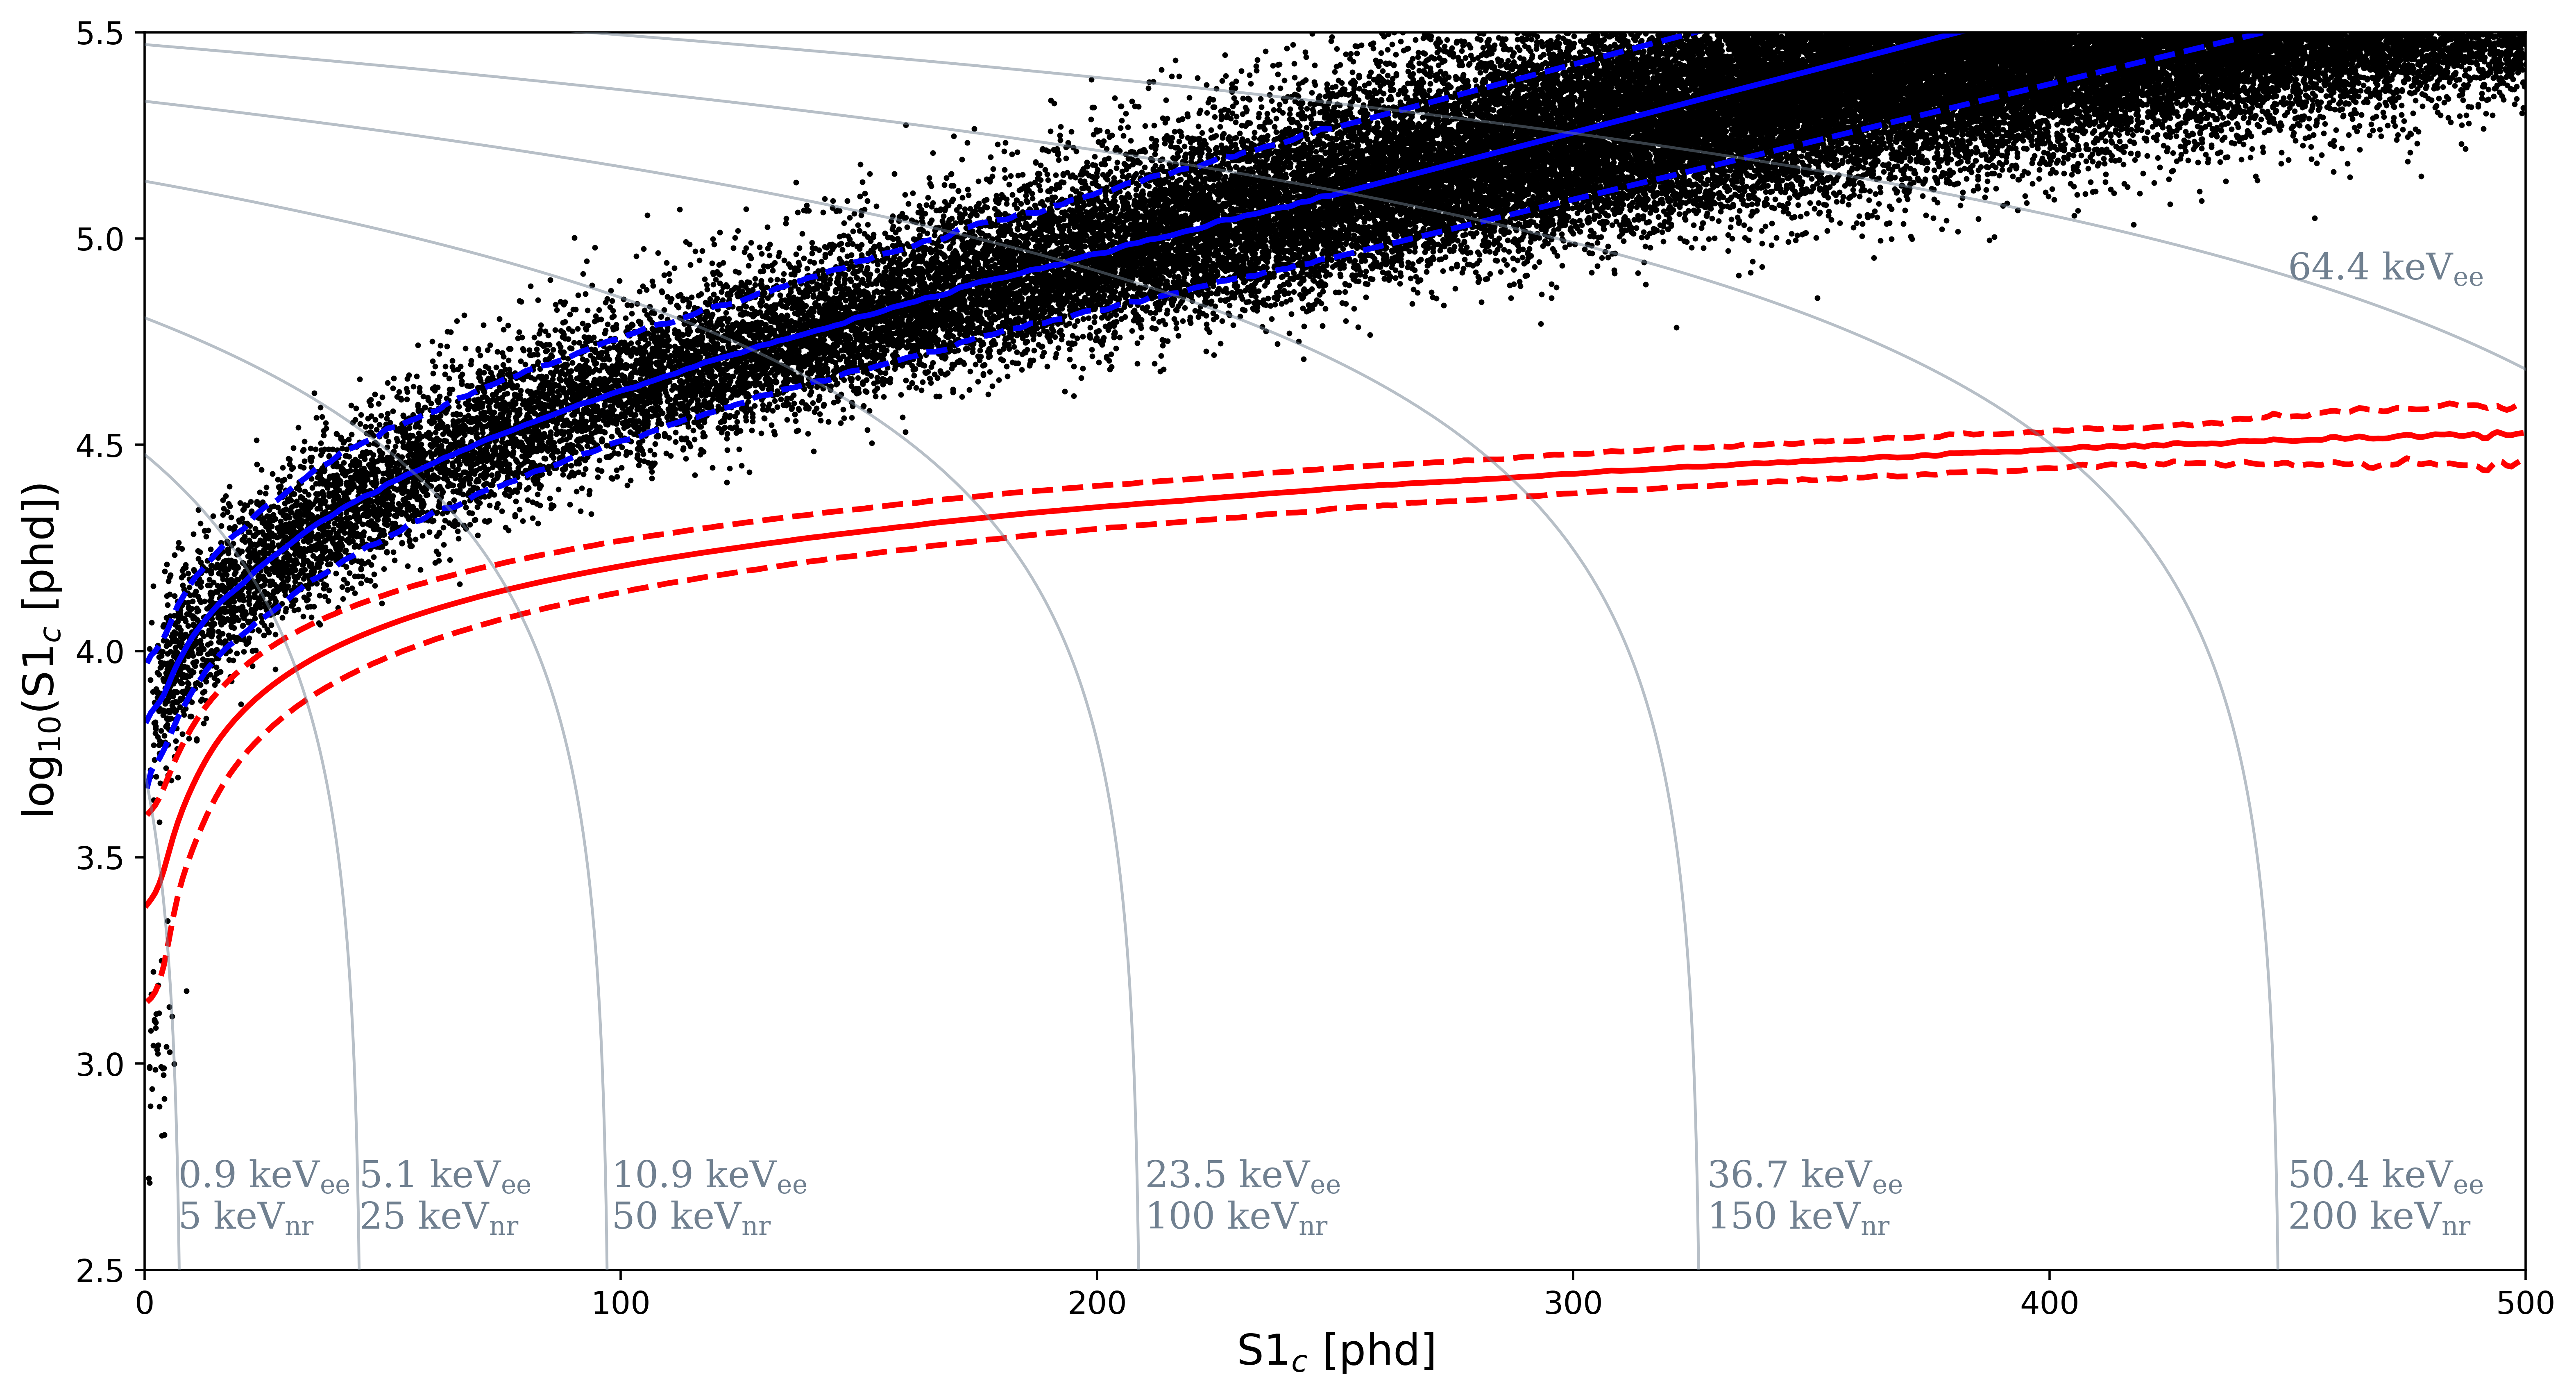
\includegraphics[width=15cm]{Figures/EFT/Projected_backgrounds/projected_backgrounds_s1_s2.png}
    \caption{Simulated data set for a background-only 1000 live day run with a 5.6 tonne fiducial mass. The ER and NR bands are shown in blue and red respectively; the solid lines are the mean and the dashed are 10\% and 90\% quantiles.}
    \label{fig:my_label}
\end{figure}







\subsection{Signal Model}
\par
\par
Both of the analyses were performed in the isoscalar basis as it allows for comparion to both LUX and XENON collraboration results.
More specifically, only the isoscalar basis was considered, with isovector interactions neglected.
\par
The case of 

\begin{equation}
    \frac{dR}{dE_R} = \frac{c^{a^2}_i \rho_\chi}{32 \pi m^3_\chi m^2_N} \int_{v_min} \frac{f(\vec{v}}{v} F^{a,a}_{i,i} (v^2, q^2) d^3 v
\end{equation}

\par
The recoil spectra were generated using \textit{DMFormFactor}.
This was chosen over the other software options mentioned in \autoref{sec:eft_theory} as it is the same as is used by the LUX, Panda-X and XENON collaborations.
Two different version of the codebase were used.
For the projected sensitivity, the recoils generated were from \textit{DMFormFactor} v6.0 which are the same version as those used in the published LUX and XENON100 results.
For the SR1 result, a newer, but unpublished version of \textit{DMFormFactor} was used\footnote{unpublished at time of writing}.
This has updated form factors, more accurately modelling the nuclei.
The recent publication on $\mathcal{L}$ by Panda-X used this version \cite{pandax_2_eft_ref}.
For a selection of operators the difference between the resultant form factors is shown in XXX.
The change in the resultant Bessel functions alter the shape of the recoils.

The WIMP signal model parameters used are shown in \autoref{tab:DMFormFactor_parameters}.
Recoil spectra out to 1000 keV for each operator were generated.

\begin{table}[]
    \centering
    \begin{tabular}{c|c}
        Parameter         & Value  \\ \hline
        $\nu_0$           & 220$km s^{-1}$ \\
        $\nu_{esc}$       & 544$km s^{-1}$ \\
        $\rho_{\chi}$     & 0.3 $GeV/cm^{3}$ \\
        $|\nu_E|$         & 245 $km s^{-1}$ 
    \end{tabular}
    \caption{DMFormFactor parameters used for the standard halo model. CITE XXX}
    \label{tab:DMFormFactor_parameters}
\end{table}
To improve the realism of the recoil and to maintain consistency with previous experiments the natural abundance of Xe isotopes were folded in.
Each operator was generated out to 1000 keV and in the isoscalar basis and a selection of the resultant differential rates are shown in \autoref{fig:HENR_Spin_Recoil_Spectrum}.
Each Operator was performed for a WIMP mass of [5, 7, 10, 12, 14, 21, 33, 50, 100, 200, 400, 1000, 4000] GeV.


\par
These were then used with the detector model to produce our observable quantities: \{$S1_c,log(S2_c)$\}, a selection of which are shown in FIGURE XXX.

%\begin{figure}[!htbp]%
\centering
    \begin{tikzpicture}
    \centering
        \begin{groupplot}[view={0}{90},
            group style = {group size = 1 by 3,
            horizontal sep=0.6cm}]
        \iffalse
        \nextgroupplot[
        width=15cm, height=8cm,
        xlabel=,
        ylabel={log$_10$(S2$_{c}$ [phd])},
        mark size=0pt,
        xmin=0, xmax=500,
        ymin=2.5, ymax=5.5,
        colormap={blackwhite}{color=(white) color=(black)}]
        
        \addplot3[
              surf,
              shader=flat corner,
        	  mesh/cols=40,
        	  mesh/ordering=rowwise,
            ] file {Data/HENR/Projected_Sensitivity/Signal/pdf/o1_m100_pdf.dat};
            
        \addplot[blue, ]
            table [x=bin, y=mean]
            {Data/HENR/Projected_Sensitivity/Signal/pdf/er_band.dat};     
        \addplot[blue, dashed]
            table [x=bin, y=high]
            {Data/HENR/Projected_Sensitivity/Signal/pdf/er_band.dat};     
        \addplot[blue, dashed]
            table [x=bin, y=low]
            {Data/HENR/Projected_Sensitivity/Signal/pdf/er_band.dat};     

        \addplot[red, ]
            table [x=bin, y=mean]
            {Data/HENR/Projected_Sensitivity/Signal/pdf/nr_band.dat};    
        \addplot[red, dashed]
            table [x=bin, y=high]
            {Data/HENR/Projected_Sensitivity/Signal/pdf/nr_band.dat};     
        \addplot[red, dashed]
            table [x=bin, y=low]
            {Data/HENR/Projected_Sensitivity/Signal/pdf/nr_band.dat};  
        
        \node[draw, fill=white] at (axis cs: 450,3) {\large $\Operator$1};    
        
        \fi
        \nextgroupplot[
        width=15cm, height=8cm,
        xlabel=,
        ylabel={log$_10$(S2$_{c}$ [phd])},
        mark size=0pt,
        xmin=0, xmax=500,
        ymin=2.5, ymax=5.5,
        colormap={blackwhite}{color=(white) color=(black)}]
        
        \addplot3[
              surf,
              shader=flat corner,
        	  mesh/cols=40,
        	  mesh/ordering=rowwise,
            ] file {Data/HENR/Projected_Sensitivity/Signal/pdf/o6_m100_pdf.dat};
            
        \addplot[blue, ]
            table [x=bin, y=mean]
            {Data/HENR/Projected_Sensitivity/Signal/pdf/er_band.dat};     
        \addplot[blue, dashed]
            table [x=bin, y=high]
            {Data/HENR/Projected_Sensitivity/Signal/pdf/er_band.dat};     
        \addplot[blue, dashed]
            table [x=bin, y=low]
            {Data/HENR/Projected_Sensitivity/Signal/pdf/er_band.dat};     

        \addplot[red, ]
            table [x=bin, y=mean]
            {Data/HENR/Projected_Sensitivity/Signal/pdf/nr_band.dat};    
        \addplot[red, dashed]
            table [x=bin, y=high]
            {Data/HENR/Projected_Sensitivity/Signal/pdf/nr_band.dat};     
        \addplot[red, dashed]
            table [x=bin, y=low]
            {Data/HENR/Projected_Sensitivity/Signal/pdf/nr_band.dat};  
            
        \node[draw, fill=white] at (axis cs: 450,3) {\large $\Operator$6};
        
        \nextgroupplot[
        width=15cm, height=8cm,
        xlabel={S1$_{c}$ [phd]},
        ylabel={log$_10$(S2$_{c}$ [phd])},
        mark size=0pt,
        xmin=0, xmax=500,
        ymin=2.5, ymax=5.5,
        colormap={blackwhite}{color=(white) color=(black)}]
        
        \addplot3[
              surf,
              shader=flat corner,
        	  mesh/cols=40,
        	  mesh/ordering=rowwise,
            ] file {Data/HENR/Projected_Sensitivity/Signal/pdf/o15_m100_pdf.dat};
            
        \addplot[blue, ]
            table [x=bin, y=mean]
            {Data/HENR/Projected_Sensitivity/Signal/pdf/er_band.dat};     
        \addplot[blue, dashed]
            table [x=bin, y=high]
            {Data/HENR/Projected_Sensitivity/Signal/pdf/er_band.dat};     
        \addplot[blue, dashed]
            table [x=bin, y=low]
            {Data/HENR/Projected_Sensitivity/Signal/pdf/er_band.dat};     

        \addplot[red, ]
            table [x=bin, y=mean]
            {Data/HENR/Projected_Sensitivity/Signal/pdf/nr_band.dat};    
        \addplot[red, dashed]
            table [x=bin, y=high]
            {Data/HENR/Projected_Sensitivity/Signal/pdf/nr_band.dat};     
        \addplot[red, dashed]
            table [x=bin, y=low]
            {Data/HENR/Projected_Sensitivity/Signal/pdf/nr_band.dat}; 
            
        \node[draw, fill=white] at (axis cs: 450,3) {\large $\Operator$15};
        
        \end{groupplot}
    \end{tikzpicture}
    \caption{Distribution of signal models in \{S1$_c$,log$_{10}$(S2$_c$) showing the variation between operators.
             Each pdf is shown for a WIMP mass of 100 GeV.}
    \label{fig:projected_detector_model_signal_pdfs}
\end{figure}


\subsection{Limits}
\par
Presented in \autoref{fig:EFT_Result_Projected_Sensitivity_1} and \autoref{EFT_Result_Projected_Sensitivity_2} are the limits from a one-sided PLR test statistic.
This was chosen over using a two-sided test as the purpose is to determine the sensitivity of LZ to the couplings, $c^{a}_i$, not the discovery significance. 
This approach is also in line with that used for the vanilla WIMP projected sensitivity \cite{LZ_projected_sensitivity_paper_ref} and other sensitivity studies within LZ \cite{LZ_Ibles_LZStats_Thesis_ref, umituktu_thesis_ref}.
\par
Included in the figures are the XENON100 \cite{xenon100_eft_ref} and LUX \cite{LUX_RUN4_EFT_2021} limits.
The parameter space which the LZ detector is a significant step forward compared to current limits.
The planned LZ exposure is orders of magnitude greater than the both LUX and XENON100 results, with 5.6 tonnes $\times$ 1000 live days for LZ compared to 34 kg $\times$ 224.6 live days with XENON100 and 100 kg $\times$ 311.2 live days for LUX.

$c^a_i$ has dimensional of mass$^{-2}$ which is 

The upper limits are shown in \autoref{fig:EFT_Result_Projected_Sensitivity_1} and \autoref{EFT_Result_Projected_Sensitivity_2}.
Note that the limit is presented in terms of the dimensionless values $({c}^{s}_{i}\times{m}^{2}_{w})^{2}$ rather than just $({c}^{s}_{i}$ (which has dimensionality of [mass]$^{-2}$, where $m_w$ is the Higg's vacuum expectation value.
This decision has been made due to several experiments making the decision to present them in this way (starting with XENON100 \cite{xenon100_eft_ref}).
\par
A key benefit of presenting in this manor is that it allows for a direct comparison to previous results which have been included in the limits shown.
Only a single data point is shown from LUX as their analysis was originally done in an \{$n,p$\} basis \cite{LUX_RUN4_EFT_2021}, and given the huge quantity of work it took they decided to reduce the problem to a single WIMP mass per operator.
\par
LZ has the potential to make significant strides in this region of parameter space which can be interpreted as 

\begin{figure}[!htbp]%
\centering
\begin{tikzpicture}
\centering
  \begin{groupplot}[view={0}{90},
    group style = {group size = 2 by 4,
                   vertical sep=1.5cm,
                   horizontal sep=2.0cm}]
    
    \pgfplotsforeachungrouped \x in {1,3,4,5,6,7,8,9}{
     \edef\tmp{
        \noexpand \nextgroupplot[
                                xlabel=Mass (MeV),
                                ylabel=$({c}^{s}_{\x}\times{m}^{2}_{w})^{2}$,
                                mark size=0pt,
                                width=0.45\textwidth,
                                height=5.5cm,
                                xmode=log,
                                ymode=log,
                                yminorticks=true,
                                x label style={at={(axis description cs:0.75,-0.1)},anchor=near ticklabel},
                                y label style={at={(axis description cs:-0.13,.75)},anchor=near ticklabel},
                                ]
            
            \noexpand \addplot[blue, name path = xenon100] table[]
                      {Data/HENR/Xenon100/O\x.dat};
                        
            \noexpand \addplot[only marks, mark size=1, error bars/.cd,
                               y dir=both, y explicit, error bar style={color=black}]
                               table[x=mass,y=median, y error plus index=3, y error minus index=2] {Data/HENR/Projected_Sensitivity/LUX/O\x.dat};
            
            \noexpand \addplot[green, opacity = 0.4, name path = nsig1] table[x=mass, y=nsig1]
                      {Data/HENR/Projected_Sensitivity/Results_method1/O\x.dat};
                      
            \noexpand \addplot[green, opacity = 0.4, name path = psig1] table[x=mass, y=psig1]
                      {Data/HENR/Projected_Sensitivity/Results_method1/O\x.dat};
                      
            \noexpand \addplot[yellow, opacity = 0.4, name path = psig2] table[x=mass, y=psig2]
                      {Data/HENR/Projected_Sensitivity/Results_method1/O\x.dat};
                      
            \noexpand \addplot[green, opacity = 0.4, forget plot] fill between[of=nsig1 and psig1];
            \noexpand \addplot[yellow, opacity = 0.4, forget plot] fill between[of=psig1 and psig2];
            
            \noexpand \addplot[black, name path = median] table[x=mass, y=median]
                      {Data/HENR/Projected_Sensitivity/Results_method1/O\x.dat};
            
            %\noexpand \addplot[black, dashed, name path = median] table[x=mass, y=cl]
            %          {Data/HENR/Projected_Sensitivity/Results/O\x.dat};
                     
        }
        \tmp 
        }
  \end{groupplot}
\end{tikzpicture}
\caption{}
\label{fig:EFT_Result_Projected_Sensitivity_1}
\end{figure}



\begin{figure}[!htbp]%
\centering
\begin{tikzpicture}
\centering
  \begin{groupplot}[view={0}{90},
    group style = {group size = 2 by 3,
                   vertical sep=1.5cm,
                   horizontal sep=2.0cm}]
    
    \pgfplotsforeachungrouped \x in {10,11,12,13,14,15}{
     \edef\tmp{
        \noexpand \nextgroupplot[
                                xlabel=Mass (MeV),
                                ylabel=$({c}^{s}_{\x}\times{m}^{2}_{w})^{2}$,
                                mark size=0pt,
                                width=0.45\textwidth,
                                height=5.5cm,
                                xmode=log,
                                ymode=log,
                                x label style={at={(axis description cs:0.75,-0.1)},anchor=near ticklabel},
                                y label style={at={(axis description cs:-0.13,.75)},anchor=near ticklabel},
                                ]
            
            \noexpand \addplot[blue, name path = xenon100] table[]
                      {Data/HENR/Xenon100/O\x.dat};
            
            \noexpand \addplot[only marks, mark size=1, error bars/.cd,
                               y dir=both, y explicit, error bar style={color=black}]
                               table[x=mass,y=median, y error plus index=3, y error minus index=2] {Data/HENR/Projected_Sensitivity/LUX/O\x.dat};
                        
            \noexpand \addplot[green, opacity = 0.4, name path = nsig1] table[x=mass, y=nsig1]
                      {Data/HENR/Projected_Sensitivity/Results_method1/O\x.dat};
                      
            \noexpand \addplot[green, opacity = 0.4, name path = psig1] table[x=mass, y=psig1]
                      {Data/HENR/Projected_Sensitivity/Results_method1/O\x.dat};
                      
            \noexpand \addplot[yellow, opacity = 0.4, name path = psig2] table[x=mass, y=psig2]
                      {Data/HENR/Projected_Sensitivity/Results_method1/O\x.dat};
                      
            \noexpand \addplot[green, opacity = 0.4, forget plot] fill between[of=nsig1 and psig1];
            \noexpand \addplot[yellow, opacity = 0.4, forget plot] fill between[of=psig1 and psig2];
            
            \noexpand \addplot[black, name path = median] table[x=mass, y=median]
                      {Data/HENR/Projected_Sensitivity/Results_method1/O\x.dat};
            
            %\noexpand \addplot[black, dashed, name path = median] table[x=mass, y=cl]
            %          {Data/HENR/Projected_Sensitivity/Results/O\x.dat};
                     
        }
        \tmp 
        }
  \end{groupplot}
\end{tikzpicture}
\caption{}
\label{fig:EFT_Result_Projected_Sensitivity}
\end{figure}
